\begin{table}[htdp]
\caption{Results for the inverse problem. The process begins with the top hat response function and computes the amplitudes $c_{0}, c_{2}, \dots, c_{n}$}
\begin{center}
\begin{tabular}{ccc}
 %
         & $\Upsilon(b)$ (fit, black) & $\psi(r)$ (reconstructed, black) \\
   order $n$ & $Y(b)$ (input, gray) & $\psi(r)$ (input, gray) \\\hline
 %
   $n = 10$ &
   \raisebox{-0.5\height}{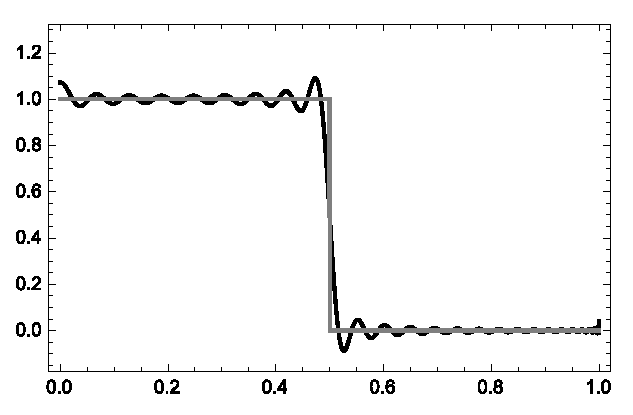
\includegraphics[ width = 2in ]{graphics/"top hat"/fit_100.eps}} &
   \raisebox{-0.5\height}{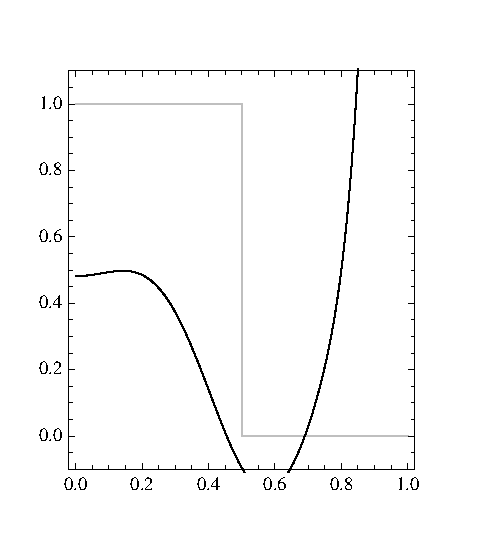
\includegraphics[ width = 2in ]{graphics/intensity_10.eps}} \\
 %
   $n = 40$ &
   \raisebox{-0.5\height}{\includegraphics[ width = 2in ]{graphics/fit_20.eps}} &
   \raisebox{-0.5\height}{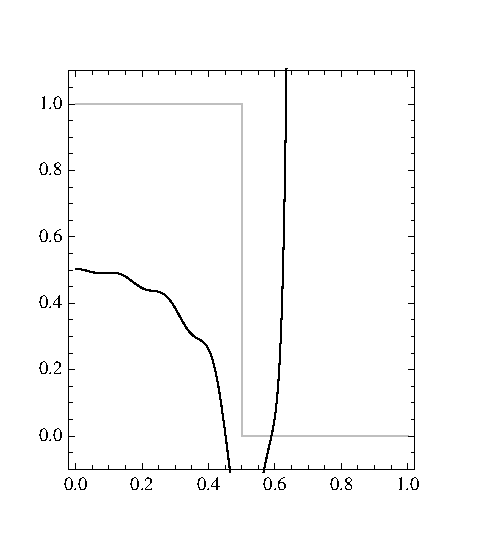
\includegraphics[ width = 2in ]{graphics/intensity_40.eps}} \\
 %
 %
 %
 %
 %
\end{tabular}
\end{center}
\label{tab:top hat results}
\end{table}%

\endinput %-------------------------------